% Vibe Shuffle — plain-language flowcharts (no formulas, no jargon).
% Build:  npm run flowcharts   (-> docs/flowcharts.pdf)
\documentclass[a4paper,11pt]{article}

\usepackage[top=1.6cm,bottom=1.4cm,left=1.6cm,right=1.6cm]{geometry}
\usepackage{xcolor}
\usepackage{tikz}
\usetikzlibrary{arrows.meta, positioning}

\pagestyle{empty}
\setlength{\parindent}{0pt}

% --- Friendly palette ------------------------------------------------------
\definecolor{happy}{HTML}{34D399}   % happy / lively
\definecolor{relaxed}{HTML}{22D3EE} % calm
\definecolor{tense}{HTML}{FB923C}   % tense
\definecolor{sadlow}{HTML}{A78BFA}  % sad
\definecolor{hrv}{HTML}{F87171}     % heartbeat channel
\definecolor{face}{HTML}{38BDF8}    % face channel
\definecolor{song}{HTML}{F59E0B}    % song channel
\definecolor{boxbg}{HTML}{F8FAFC}
\definecolor{boxbd}{HTML}{CBD5E1}
\definecolor{ink}{HTML}{1E293B}
\definecolor{soft}{HTML}{64748B}

\colorlet{accent}{hrv}

\tikzset{
  box/.style={rectangle, rounded corners=6pt, draw=boxbd, line width=0.7pt,
              fill=boxbg, align=center, inner sep=9pt, text width=10.6cm,
              text=ink, font=\small},
  result/.style={box, fill=accent!16, draw=accent, line width=1pt},
  mini/.style={rectangle, rounded corners=6pt, align=center, inner sep=6pt,
               text width=3.0cm, font=\small, text=ink},
  mode/.style={rectangle, rounded corners=6pt, draw=boxbd, line width=0.8pt,
               align=center, inner sep=8pt, text width=6.4cm, font=\small,
               text=ink},
  num/.style={circle, fill=accent, text=white, font=\bfseries\small,
              minimum size=7.5mm, inner sep=0pt},
  arrow/.style={-{Stealth[length=3mm]}, line width=0.9pt, draw=soft},
}

% headline of a box: bold title, then plain explanation underneath
\newcommand{\head}[1]{{\normalsize\bfseries #1}\\[3pt]}

\newcommand{\charttitle}[2]{%
  \begin{center}
    {\LARGE\bfseries #1}%
    \def\tmpsub{#2}\ifx\tmpsub\empty\else\\[4pt]{\small\color{soft} #2}\fi
  \end{center}
  \vspace{4mm}}

% a horizontal "from ... to ..." scale bar
\newcommand{\scalebar}[4]{% leftcolor, rightcolor, leftlabel, rightlabel
  \begin{tikzpicture}
    \shade[left color=#1!45, right color=#2!75, rounded corners=6pt]
      (0,0) rectangle (11,0.8);
    \draw[rounded corners=6pt, draw=boxbd] (0,0) rectangle (11,0.8);
    \node[font=\small\bfseries, text=ink, anchor=base] at (1.7,0.33) {#3};
    \node[font=\small\bfseries, text=ink, anchor=base] at (9.2,0.33) {#4};
    \node[font=\large, text=soft, anchor=base] at (5.5,0.33) {$\longleftrightarrow$};
  \end{tikzpicture}}

\begin{document}

% =========================================================================
% PAGE 1 — Heartbeat -> energy level
% =========================================================================
\colorlet{accent}{hrv}
\charttitle{How your heartbeat becomes an ``energy'' level}{}

\begin{center}
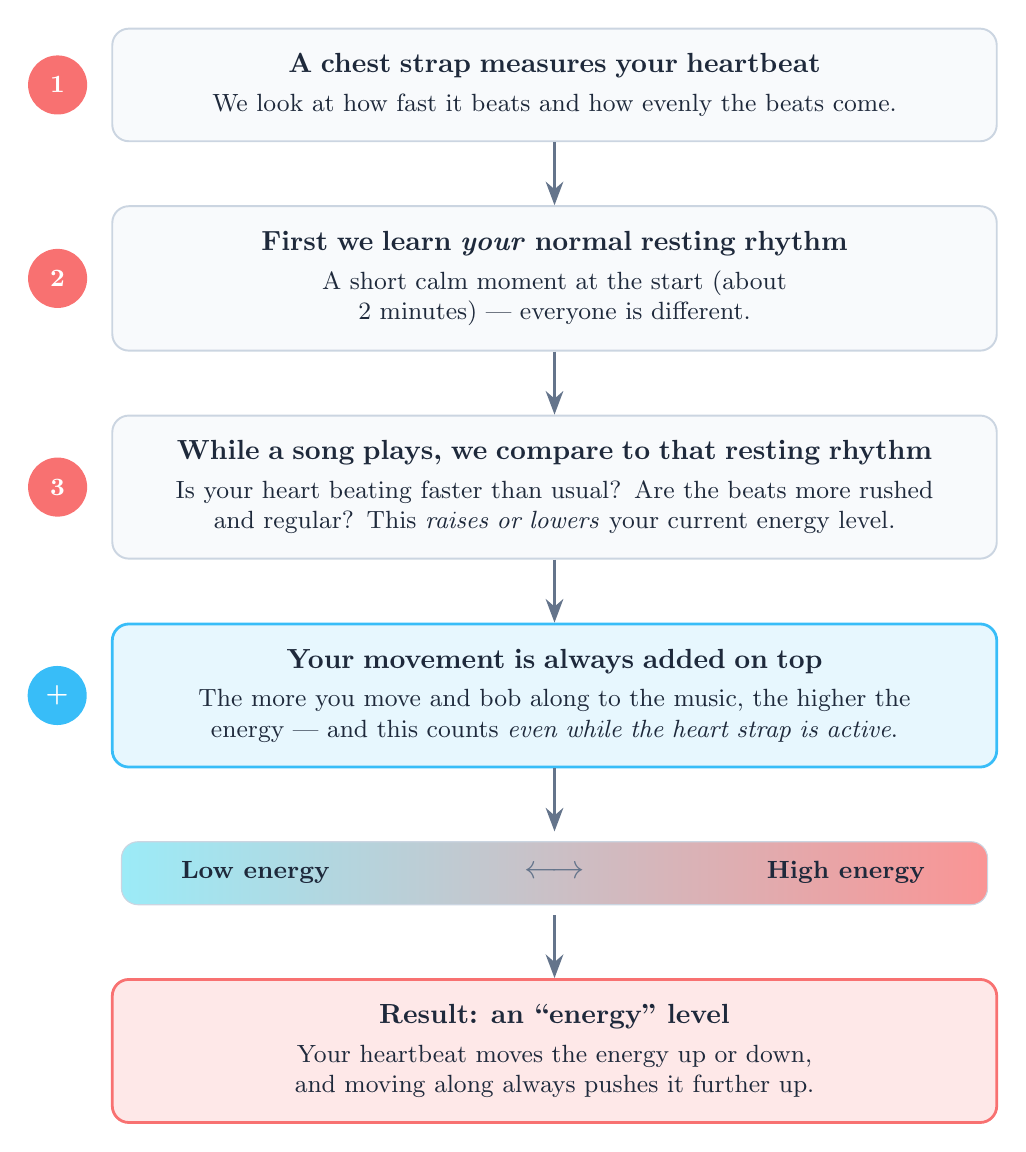
\begin{tikzpicture}[node distance=8mm]
  \node[box] (b1)
    {\head{A chest strap measures your heartbeat}
     We look at how fast it beats and how evenly the beats come.};
  \node[box, below=of b1] (b2)
    {\head{First we learn \emph{your} normal resting rhythm}
     A short calm moment at the start (about 2 minutes) — everyone is different.};
  \node[box, below=of b2] (b3)
    {\head{While a song plays, we compare to that resting rhythm}
     Is your heart beating faster than usual? Are the beats more rushed and
     regular? This \emph{raises or lowers} your current energy level.};
  \node[box, fill=face!12, draw=face, line width=1pt, below=of b3] (bmove)
    {\head{Your movement is always added on top}
     The more you move and bob along to the music, the higher the energy~--- and
     this counts \emph{even while the heart strap is active}.};
  \node[below=8mm of bmove] (bar) {\scalebar{relaxed}{hrv}{Low energy}{High energy}};
  \node[result, below=8mm of bar] (b5)
    {\head{Result: an ``energy'' level}
     Your heartbeat moves the energy up or down, and moving along always pushes
     it further up.};

  \node[num, left=3mm of b1] {1};
  \node[num, left=3mm of b2] {2};
  \node[num, left=3mm of b3] {3};
  \node[num, fill=face, left=3mm of bmove] {+};

  \draw[arrow] (b1) -- (b2);
  \draw[arrow] (b2) -- (b3);
  \draw[arrow] (b3) -- (bmove);
  \draw[arrow] (bmove) -- (bar);
  \draw[arrow] (bar) -- (b5);
\end{tikzpicture}
\end{center}

\newpage

% =========================================================================
% PAGE 2 — Face -> mood level
% =========================================================================
\colorlet{accent}{face}
\charttitle{How your face becomes a ``mood'' level}{}

\begin{center}
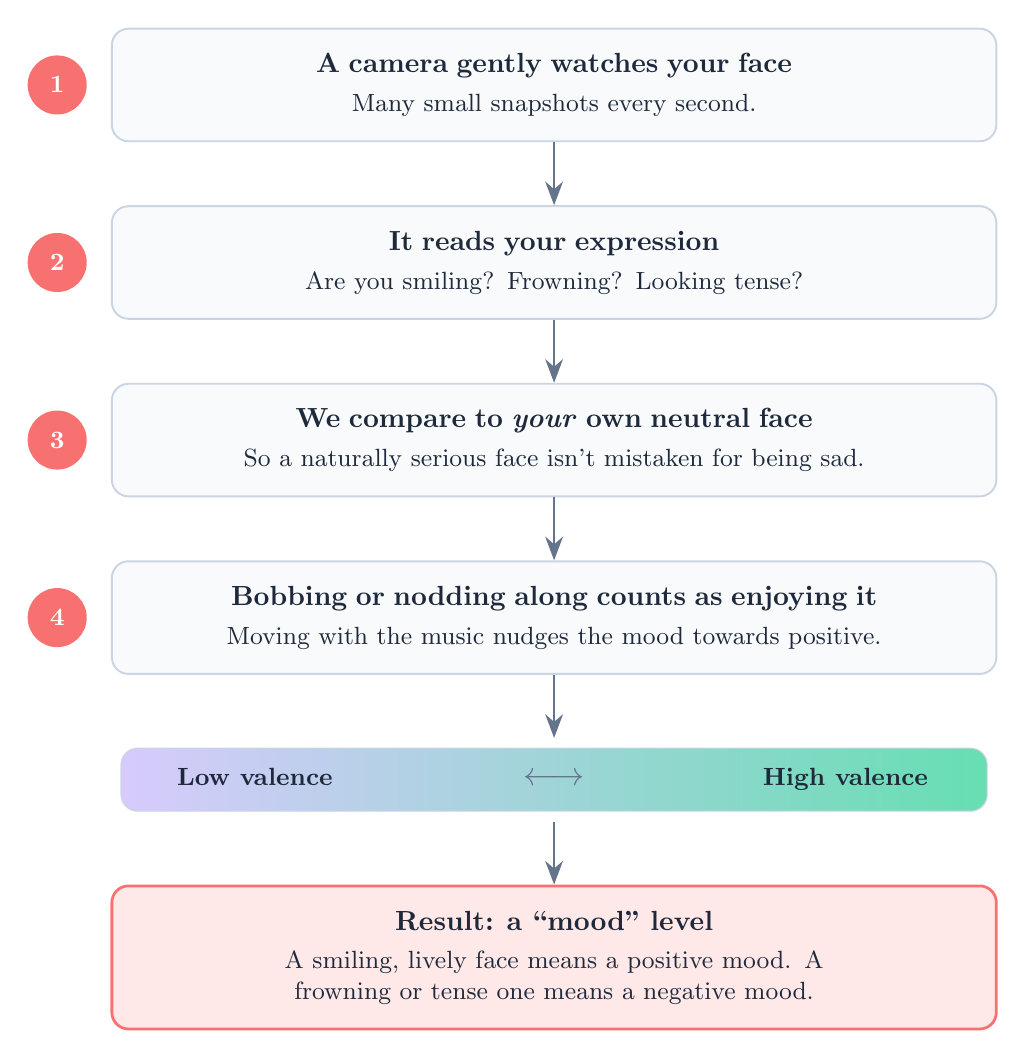
\begin{tikzpicture}[node distance=8mm]
  \node[box] (b1)
    {\head{A camera gently watches your face}
     Many small snapshots every second.};
  \node[box, below=of b1] (b2)
    {\head{It reads your expression}
     Are you smiling? Frowning? Looking tense?};
  \node[box, below=of b2] (b3)
    {\head{We compare to \emph{your} own neutral face}
     So a naturally serious face isn't mistaken for being sad.};
  \node[box, below=of b3] (b4)
    {\head{Bobbing or nodding along counts as enjoying it}
     Moving with the music nudges the mood towards positive.};
  \node[below=8mm of b4] (bar) {\scalebar{sadlow}{happy}{Low valence}{High valence}};
  \node[result, below=8mm of bar] (b6)
    {\head{Result: a ``mood'' level}
     A smiling, lively face means a positive mood. A frowning or tense one
     means a negative mood.};

  \node[num, left=3mm of b1] {1};
  \node[num, left=3mm of b2] {2};
  \node[num, left=3mm of b3] {3};
  \node[num, left=3mm of b4] {4};

  \draw[arrow] (b1) -- (b2);
  \draw[arrow] (b2) -- (b3);
  \draw[arrow] (b3) -- (b4);
  \draw[arrow] (b4) -- (bar);
  \draw[arrow] (bar) -- (b6);
\end{tikzpicture}
\end{center}

\newpage

% =========================================================================
% PAGE 3 — Songs: where the 100 come from & how one is chosen
% =========================================================================
\colorlet{accent}{song}
\charttitle{Where the 100 songs come from, and how one is chosen}
          {Built once at the start; one song picked at a time}

\begin{center}
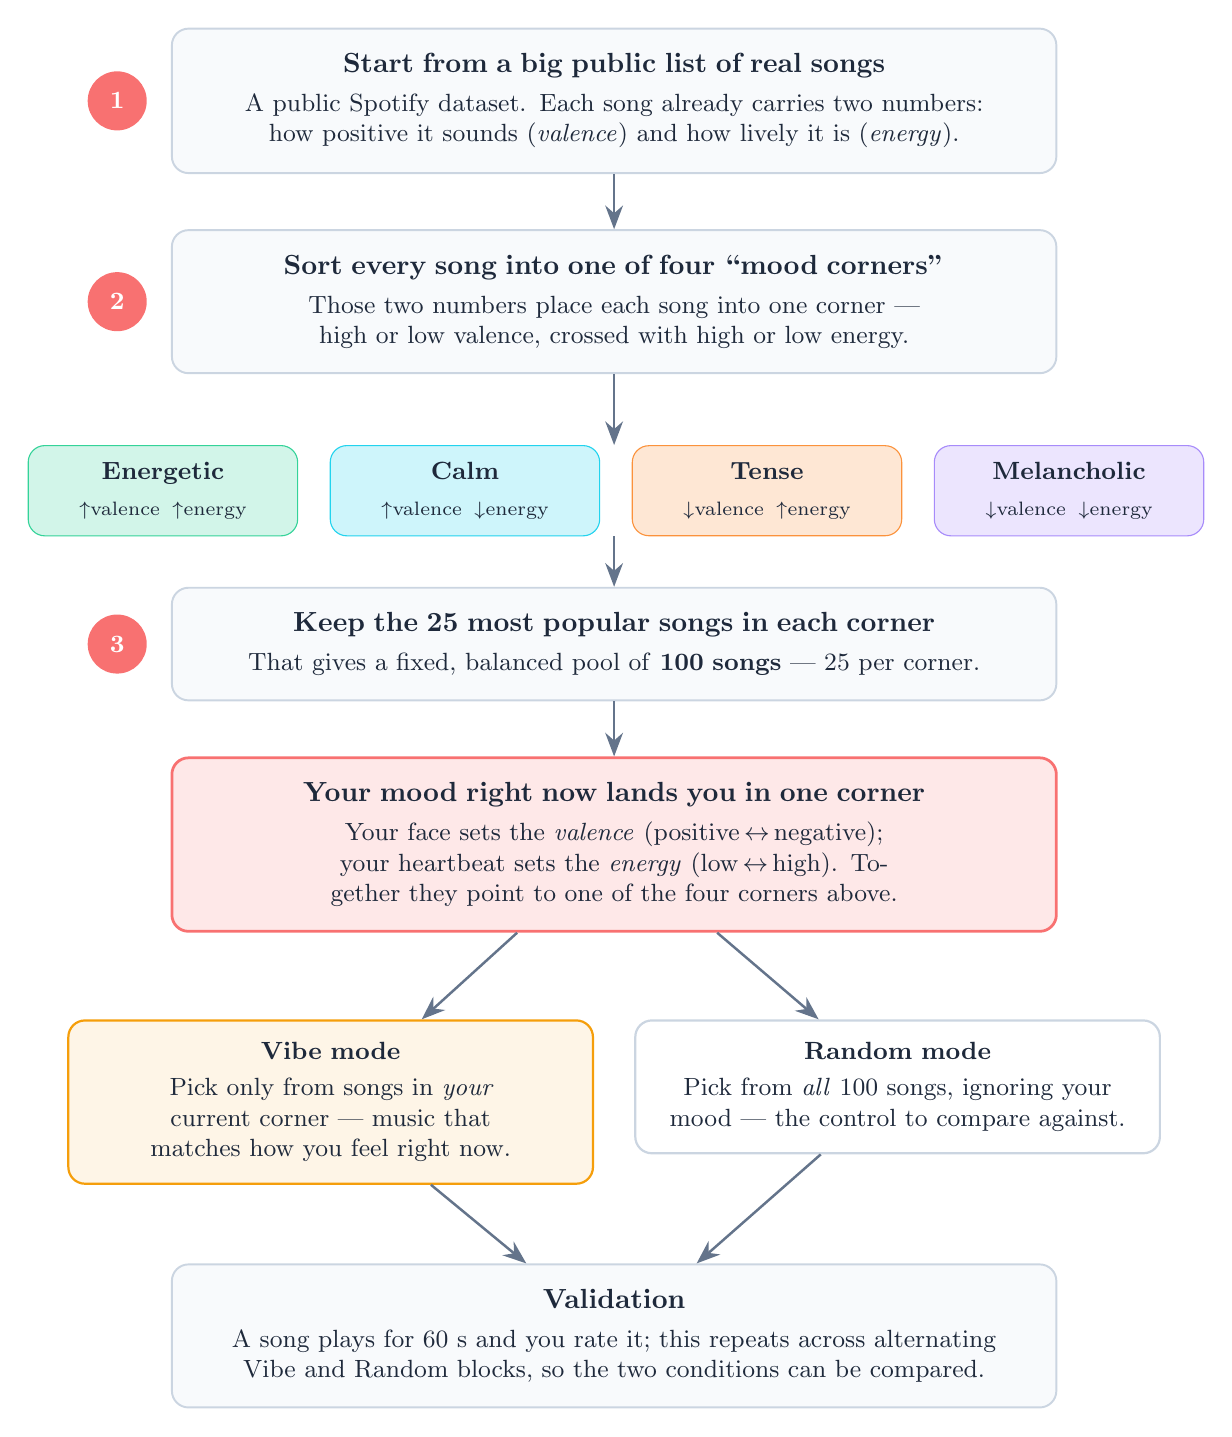
\begin{tikzpicture}[node distance=7mm]
  % ---- Part A: building the pool ----
  \node[box] (a1)
    {\head{Start from a big public list of real songs}
     A public Spotify dataset. Each song already carries two numbers: how
     positive it sounds (\emph{valence}) and how lively it is (\emph{energy}).};
  \node[box, below=of a1] (a2)
    {\head{Sort every song into one of four ``mood corners''}
     Those two numbers place each song into one corner --- high or low valence,
     crossed with high or low energy.};

  % four colored corner chips (standard quadrant names + axis hint)
  \node[mini, fill=happy!22, draw=happy, below=9mm of a2, xshift=-5.73cm] (c1)
    {\textbf{Energetic}\\[2pt]{\scriptsize $\uparrow$valence\, $\uparrow$energy}};
  \node[mini, fill=relaxed!22, draw=relaxed, right=4mm of c1] (c2)
    {\textbf{Calm}\\[2pt]{\scriptsize $\uparrow$valence\, $\downarrow$energy}};
  \node[mini, fill=tense!22, draw=tense, right=4mm of c2] (c3)
    {\textbf{Tense}\\[2pt]{\scriptsize $\downarrow$valence\, $\uparrow$energy}};
  \node[mini, fill=sadlow!22, draw=sadlow, right=4mm of c3] (c4)
    {\textbf{Melancholic}\\[2pt]{\scriptsize $\downarrow$valence\, $\downarrow$energy}};

  \node[box, below=27mm of a2] (a3)
    {\head{Keep the 25 most popular songs in each corner}
     That gives a fixed, balanced pool of \textbf{100 songs} --- 25 per corner.};

  % ---- Part B: the validation experiment ----
  \node[result, below=of a3] (b1)
    {\head{Your mood right now lands you in one corner}
     Your face sets the \emph{valence} (positive\,$\leftrightarrow$\,negative);
     your heartbeat sets the \emph{energy} (low\,$\leftrightarrow$\,high).
     Together they point to one of the four corners above.};

  \node[mode, fill=song!10, draw=song, text width=6.1cm,
        below=11mm of b1, xshift=-3.6cm] (vibe)
    {\textbf{Vibe mode}\\[2pt]
     Pick only from songs in \emph{your} current corner --- music that matches
     how you feel right now.};
  \node[mode, text width=6.1cm, below=11mm of b1, xshift=3.6cm] (rand)
    {\textbf{Random mode}\\[2pt]
     Pick from \emph{all} 100 songs, ignoring your mood --- the control to
     compare against.};

  \node[box, below=42mm of b1] (pick)
    {\head{Validation}
     A song plays for 60 s and you rate it; this repeats across alternating
     Vibe and Random blocks, so the two conditions can be compared.};

  \node[num, left=3mm of a1] {1};
  \node[num, left=3mm of a2] {2};
  \node[num, left=3mm of a3] {3};

  \draw[arrow] (a1) -- (a2);
  \draw[arrow] (a2) -- (c2.north -| a2);
  \draw[arrow] (c2.south -| a3) -- (a3);
  \draw[arrow] (a3) -- (b1);
  \draw[arrow] (b1) -- (vibe);
  \draw[arrow] (b1) -- (rand);
  \draw[arrow] (vibe) -- (pick);
  \draw[arrow] (rand) -- (pick);
\end{tikzpicture}
\end{center}

\end{document}
